\subsection*{Арифметика в кольце, комбинаторика, функция Эйлера [7] }
\begin{center}
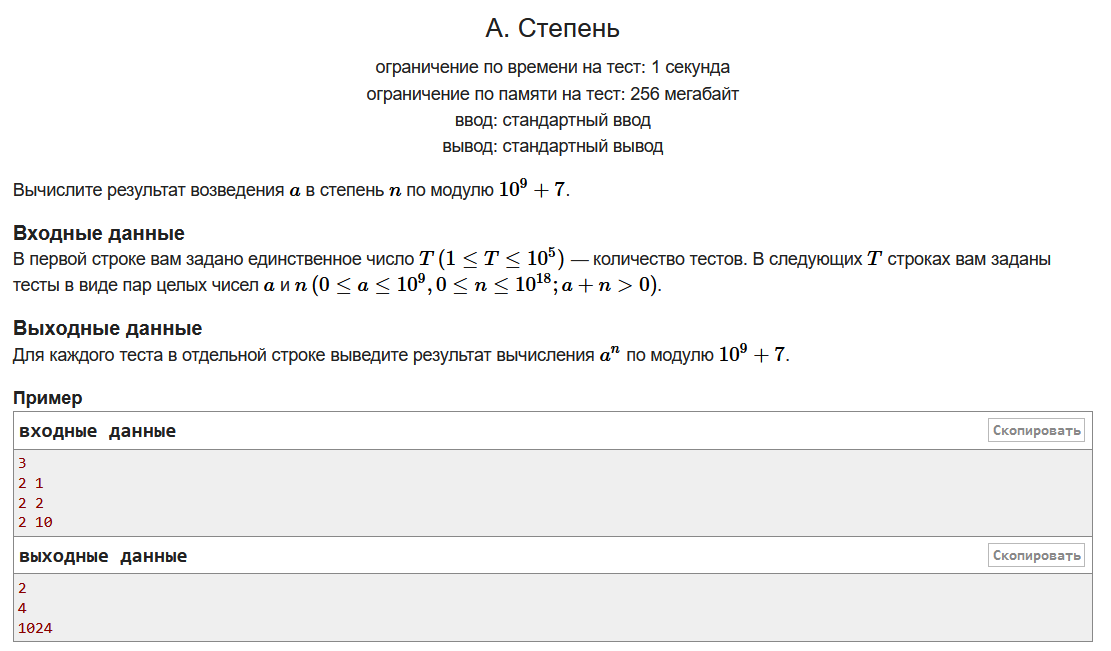
\includegraphics[width=\textwidth]{9A.png}
\end{center}
\subsubsection*{Идея решения}
Реализуем логарифмическое возведение в степень: от степени n мы переходим, если она чётна, к $n / 2$, а иначе — к $n-1$. Понятно, что всего будет не более $2 \log n$ переходов, прежде чем мы придём к $n = 0$. К тому же, после каждого перемножения будем брать остаток по $m=10^9+7$.
\subsubsection*{Исходный код}
\begin{lstlisting}
#include <iostream>
#include <string>
#include <unordered_map>
#include <unordered_set>
#include <map>
#include <set>
#include <algorithm>
#include <vector>
#include <cmath>
#include <numeric>
#include <iomanip>
#include <stack>
#include <fstream>
using namespace std;
typedef long long ll;
ll mod = 1000000007;
int main()
{
    ios_base::sync_with_stdio(false);
    cin.tie(0);
    cout.tie(0);
    ll t;
    cin >> t;
    for (int _ = 0; _ < t; _++) {
        ll res = 1;
        ll a, n;
        cin >> a >> n;
        while (n > 0) {
            if (n % 2 == 1) {
                res = (res * a) % mod;
            }
            a = (a * a) % mod;
            n /= 2;
        }
        cout << res << endl;
    }
    return 0;
}
\end{lstlisting}
\subsubsection*{Фрагмент турнирной таблицы контеста}
\begin{center}
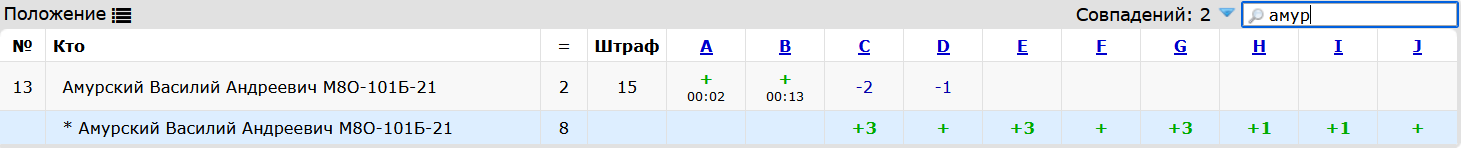
\includegraphics[width=\textwidth]{state9.png}\newline\noindent
\end{center}

\subsubsection*{Выводы}
Задача решена, проблем не возникло.
